\documentclass[10pt]{beamer}	
%\documentclass[10pt,aspectratio=43,mathserif]{beamer}		
%设置为 Beamer 文档类型,设置字体为 10pt,长宽比为16:9,数学字体为 serif 风格
%\documentclass[handout]{beamer}

\usepackage{seu}
\usepackage{amsmath,amsfonts,amssymb,bm}
\usepackage{color}
\usepackage{graphicx,hyperref,url}	
\usepackage[utf8]{inputenc}
\usepackage[main=english]{babel} 

\title[\textbf{Operating System Concepts}]{\textbf{OPERATING SYSTEM CONCEPTS}}
\subtitle{\textbf{Chapter 1. Introduction}}
\author{\textbf{A/Prof. Kai Dong}}

\institute[CSE@SEU]{
{dk@seu.edu.cn}\\
  School of Computer Science and Engineering,\\Southeast University}

\date{\scriptsize \today}

\usepackage{tikz}
\usetikzlibrary{calc, shapes, backgrounds}

% used within this chapter
\usepackage{marvosym}
\usepackage{multirow}
\usepackage{tipa}
\usepackage{url}

\usepackage{pgfgantt}
\usepackage{adjustbox}
\usepackage{colortbl}

\setbeamertemplate{itemize/enumerate body begin}{\footnotesize}
\setbeamertemplate{itemize/enumerate subbody begin}{\footnotesize}
\setbeamertemplate{itemize/enumerate subsubbody begin}{\footnotesize}

\begin{document}

\begin{frame}[label=title]
\titlepage
\end{frame}

\begin{frame}<beamer>
\frametitle{Contents}
\tableofcontents[
 sectionstyle=show/show,
 subsectionstyle=hided/hided
 ]
\end{frame}

\AtBeginSection[]{
\begin{frame}<beamer>
\frametitle{Contents}
\tableofcontents[
 sectionstyle=show/shaded,
 subsectionstyle=show/shaded
 ]
\end{frame}}

\section[0.Prologue]{Warm-up}
\begin{frame}{Warm-up}
\framesubtitle{Discussion}
\begin{itemize}
\item What Operating System(s) are you familiar with?
\item What is the best Operating System in your opinion? And for what features?
\end{itemize}
\begin{figure}
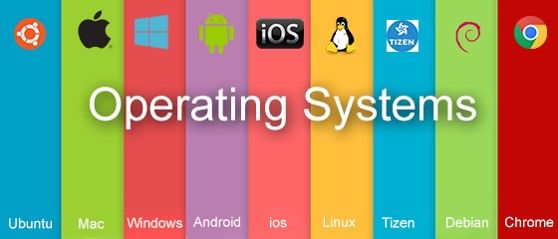
\includegraphics[width=.8\linewidth]{resources/cots_os.jpg} 
\end{figure}
\end{frame}

\begin{frame}{Objectives}
\begin{itemize}
\item To describe the basic organization of computer systems.
\item To explain the evolution of operating system structures.
\item To provide a grand tour of the major components of operating systems.
\item To give an overview of the many types of computing environments.
\item To explore several open-source operating systems.
\end{itemize}
\end{frame}

\section[1.Intro OS]{What Operating Systems Do}
\begin{frame}{What Operating Systems Do}
\framesubtitle{What is an Operating System?}
\begin{itemize}
\item A \alert{program} that acts as an intermediary between a user of a computer and the computer hardware.
\note[item]{\alert{Prefix}: Before we explore what an operating system does, we should first figure out what an operating system is.}
\note[item]{It is ...}
\item Operating system goals:
\note[item]{Operating systems mainly have three goals.}
\begin{itemize}
\item Execute user programs and make solving user problems \alert{easier}.
\item Make the computer system \alert{convenient} to use.
\item Use the computer hardware in an \alert{efficient} manner.
\end{itemize}
\note[item]{\alert{Postfix}: We now know that an operating system is a program, it has the afore-mentioned three goals. But what an operating system does?}
\end{itemize}
\end{frame}

\begin{frame}{What Operating Systems Do}
\framesubtitle{Computer System Structure}
Computer system can be divided into four components:
\begin{itemize}
\note[item]{\alert{Prefix}: We all know that an operating system is part of a computer system. Knowing what other parts of the computer system do, can help us better understand what an operating system does in the computer system.}
\item \textbf{Hardware} --- provides basic computing resources.
\begin{itemize}
\item CPU, memory, I/O devices
\end{itemize}
\item \alert{\textbf{Operating system}} --- controls and coordinates use of hardware among various applications and users
\note[item]{\alert{Postfix}: This is what operating systems do in computer systems.}
\item \textbf{Application programs} --- define the ways in which the system resources are used to solve the computing problems of the users.
\begin{itemize}
\item Word processors, compilers, web browsers, database systems, video games
\end{itemize}
\item \textbf{Users}
\begin{itemize}
\item People, machines, other computers
\end{itemize}
\end{itemize}
\end{frame}

\begin{frame}{What Operating Systems Do}
\framesubtitle{Computer System Structure (contd.)}
\begin{figure}
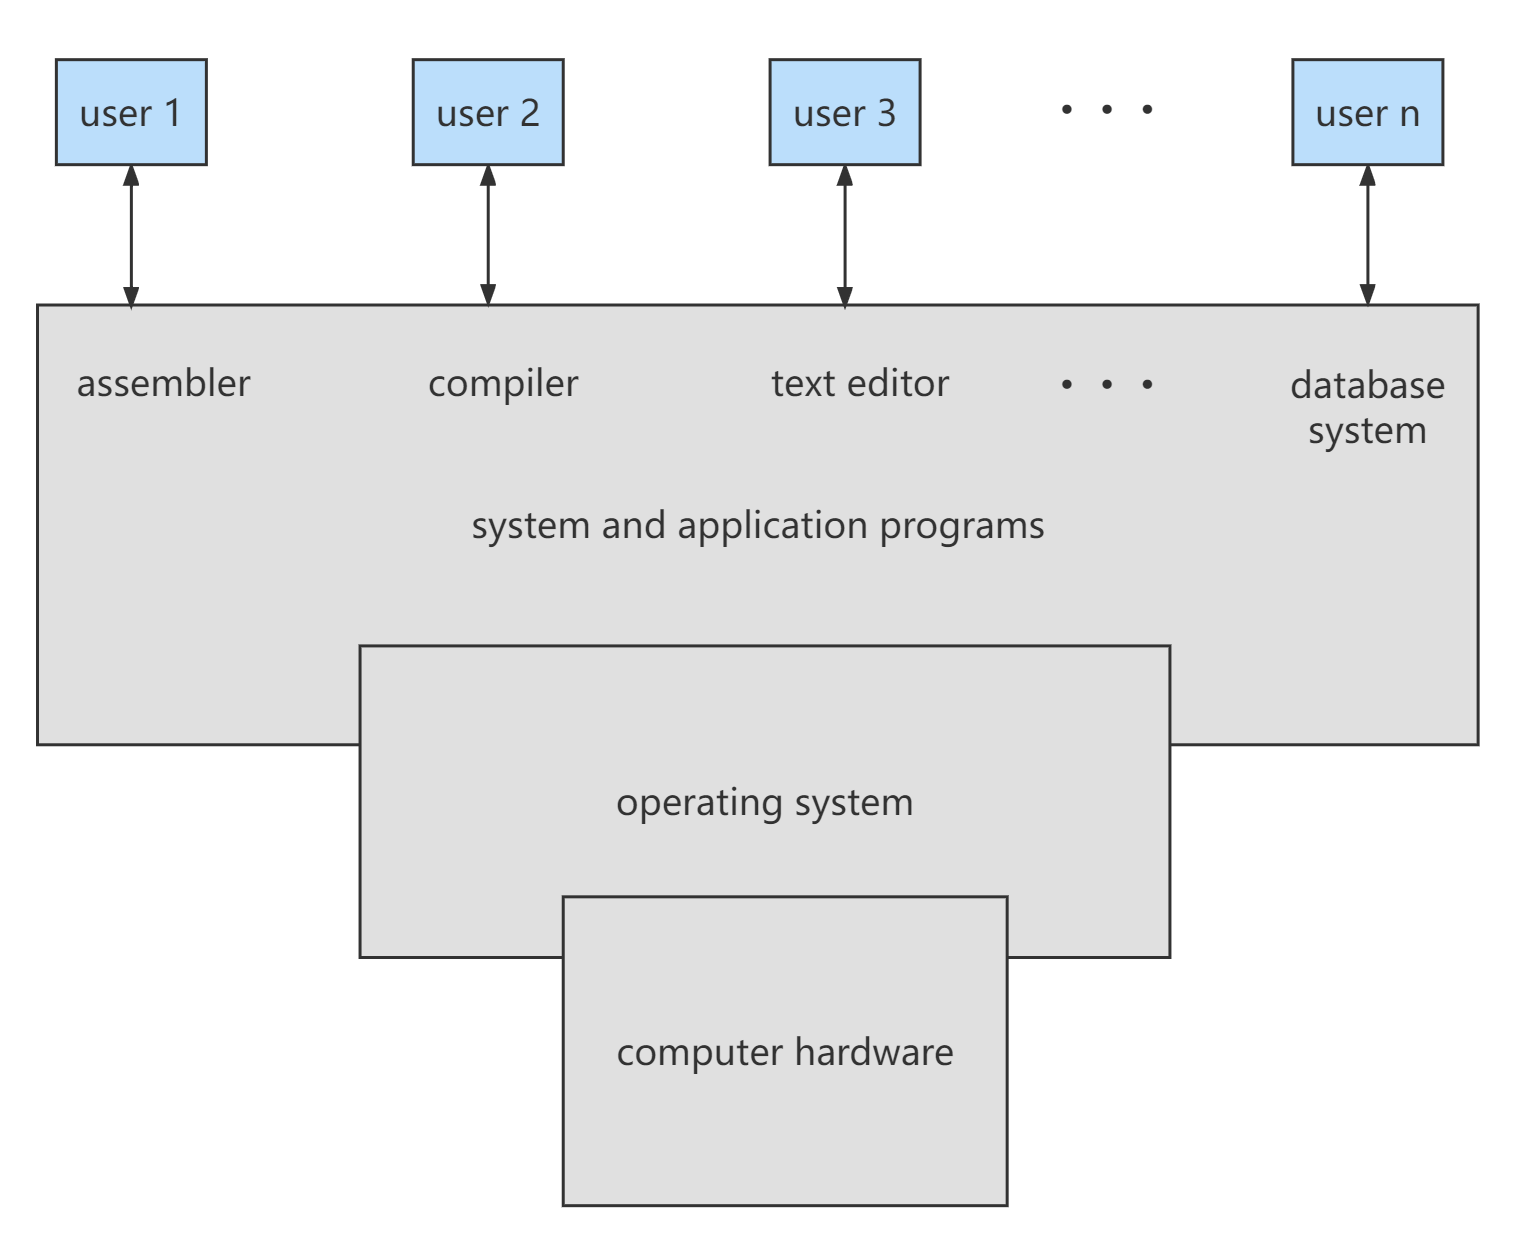
\includegraphics[width=.6\linewidth]{resources/1-7computer_system_structure.jpg} 
\end{figure}
\begin{itemize}
\item We can explore operating systems from two viewpoints: that of the \alert{user} and that of the \alert{system}.
\note[item]{\alert{Prefix}: You may have found out that ...}
\end{itemize}
\end{frame}

\begin{frame}{What Operating Systems Do}
\framesubtitle{User View}
\begin{itemize}
\note[item]{\alert{Prefix}: From the view of the user ...}
\item Want \alert{convenience}, \alert{ease of use} and \alert{good performance}. 
\item Don't care about \textcolor{blue}{resource utilization}.
\note[item]{Of cause, this is not always true. There are situations where the user also cares about resource utilization. For example, ...}
\begin{itemize}
\item But \emph{shared computer} such as \emph{mainframe} or \emph{minicomputer} must keep all users happy.
\item Users of dedicate systems such as \emph{workstations} have dedicated resources but frequently use shared resources from \emph{servers}.
\item Handheld computers are resource poor, optimized for usability and battery life.
\item Some computers have little or no user interface, such as embedded computers in devices and automobiles.
\end{itemize}
\note[item]{\alert{Postfix}: This is what operating systems do from the view of the user.}
\end{itemize}
\end{frame}

\begin{frame}{What Operating Systems Do}
\framesubtitle{System View}
\begin{itemize}
\note[item]{\alert{Prefix}: From the view of the system ...}
\item OS is a \alert{resource allocator}.
\begin{itemize}
\item Manages all resources.
\item Decides between conflicting requests for efficient and fair resource use.
\end{itemize}
\item OS is a \alert{control program}.
\begin{itemize}
\item Controls execution of programs to prevent errors and improper use of the computer.
\end{itemize}
\note[item]{\alert{Postfix}: This is what operating systems do from the view of the system.}
\end{itemize}
\end{frame}

\begin{frame}{What Operating Systems Do}
\framesubtitle{Defining Operating Systems}
\begin{itemize}
\item \alert{No universally accepted definition}.
\note[item]{\alert{Prefix}: I have talked too much on the concept of operating system. I was trying to describe this concept, but it is difficult to define it. Because there is ...}
\item ``Everything a vendor ships when you order an operating system'' 
\begin{itemize}
\item is a good approximation,
\item but varies wildly.
\end{itemize}
\item ``The one program running at all times on the computer''
\begin{itemize}
\item defines the kernel,
\item everything else is either
\begin{itemize}
\item a system program (ships with the operating system) , or
\item an application program.
\end{itemize}
\end{itemize}
\end{itemize}
\end{frame}

\section[2.Organization]{Computer-System Organization}
\begin{frame}{Computer-System Organization}
\framesubtitle{Computer Startup}
\begin{itemize}
\item \alert{Bootstrap program} is loaded at power-up or reboot.
\begin{itemize}
\item Typically stored in ROM or EPROM, generally known as firmware.
\item Initializes all aspects of system.
\item Loads operating system kernel and starts execution.
\end{itemize}
\item Think of:
\begin{itemize}
\item What happens when a program runs / How instructions are executed?
\item Millions/billions of times a second,
\begin{itemize}
\item the processor fetches an instruction from memory,
\item decodes it,
\item executes it,
\item moves on to the next till end.
\end{itemize}
\end{itemize}
\end{itemize}
\end{frame}

\begin{frame}{Computer-System Organization}
\framesubtitle{Von Neumann Model}
\begin{itemize}
\item We have just described the basics of the \alert{Von Neumann model} of computing.
\item ``… an electronic digital computer with parts consisting of 
\begin{itemize}
\item \textcolor{orange}{a processing unit containing an arithmetic logic unit and processor registers}; 
\item \textcolor{olive}{a control unit containing an instruction register and program counter}; 
\item \textcolor{green}{a memory to store both data and instructions}; 
\item \textcolor{cyan}{external mass storage}; and
\item \textcolor{violet}{input and output mechanisms}.''\\
{--- Wikipedia ``Von Neumann architecture''.}
\end{itemize}
\end{itemize}
\end{frame}

\begin{frame}{Computer-System Organization}
\framesubtitle{Von Neumann Model (contd.)}
\small
The above Von Neumann Model defines/describes:
\begin{itemize}
\small
\item How is a computer-system organized
\begin{itemize}
\item One or more CPUs, device controllers connect through common bus providing access to shared memory.
\end{itemize}
\item How is a computer-system operating
\begin{itemize}
\item Concurrent execution of CPUs and devices competing for memory cycles.
\end{itemize}
\end{itemize}
\begin{figure}
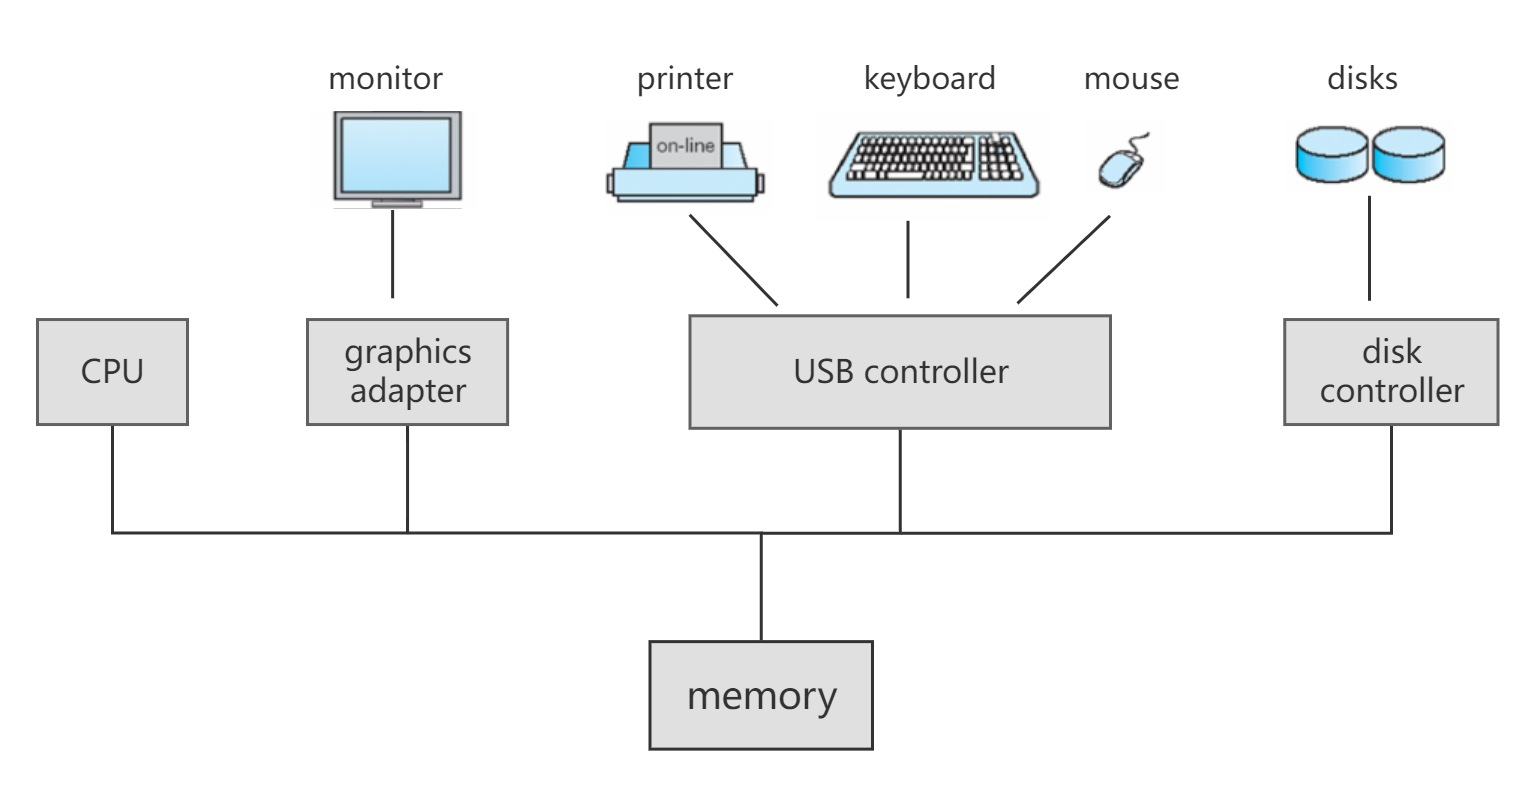
\includegraphics[width=.6\linewidth]{resources/1-14computer_system_organization.jpg} 
\end{figure}
\end{frame}

\begin{frame}{Computer-System Organization}
\framesubtitle{Computer-System Operation}
\begin{itemize}
\item I/O devices and the CPU can execute \alert{concurrently}.
\note[item]{concurrency vs. synchronization}
\item But how?
\begin{itemize}
\item Each device controller is in charge of a particular device type.
\item Each device controller has a local buffer.
\item CPU moves data from/to main memory to/from local buffers.
\item I/O is from the device to local buffer of controller.
\end{itemize}
\item By now communication is enabled, but how to cooperate?
\begin{itemize}
\item Device controller informs CPU that it has finished its operation by causing an \textbf{\alert{interrupt}}.
\end{itemize}
\note[item]{What is an interrupt? What an interrupt does?}
\end{itemize}
\end{frame}

\begin{frame}{Computer-System Organization}
\framesubtitle{Common Functions of Interrupts}
\begin{itemize}
\item An interrupt is an input signal to the processor indicating an event that needs immediate attention.
\item Interrupt transfers \textbf{control} to the interrupt service routine generally, through the \textbf{\alert{interrupt vector}}, which contains the addresses of all the service routines.
\note[item]{What is an interrupt vector?}
\item Interrupt architecture must save the address of the interrupted instruction.
\item A \textbf{\alert{trap}} or \textbf{\alert{exception}} is a software-generated interrupt caused either by an error or a user request.
\item An operating system is \textbf{\alert{interrupt driven}}.
\note[item]{What is interrupt driven?}
\end{itemize}
\end{frame}

\begin{frame}{Computer-System Organization}
\framesubtitle{Interrupt Handling}
\begin{itemize}
\note[item]{\alert{Prefix}: When an interrupt takes place, how to handle it?}
\item The operating system preserves the state of the CPU by storing registers and the program counter.
\item Determines which type of interrupt has occurred:
\begin{itemize}
\item \alert{polling}, or
\item \alert{vectored} interrupt system
\end{itemize}
\item Separate segments of code determine what action should be taken for each type of interrupt.
\end{itemize}
\end{frame}

% \begin{frame}{Computer-System Organization}
% \framesubtitle{Interrupt Timeline}
% \begin{figure}
% 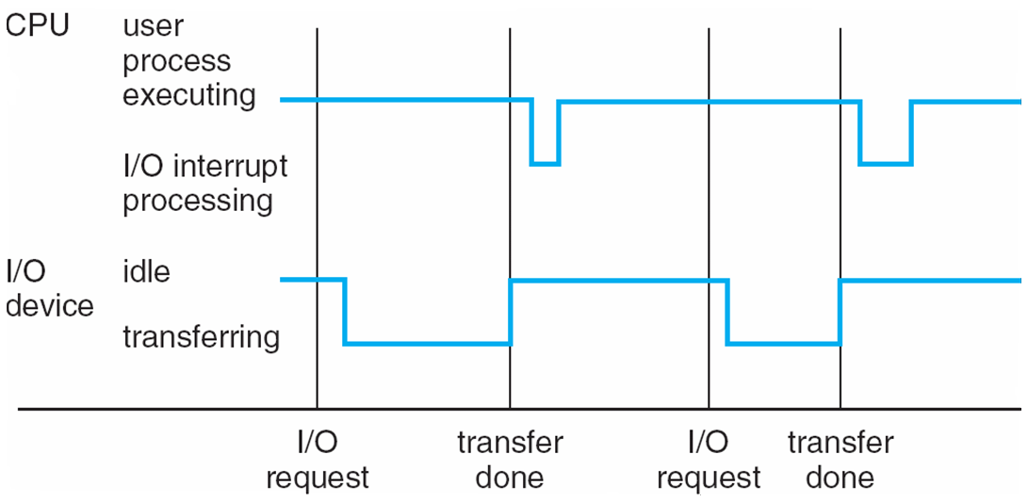
\includegraphics[width=.8\linewidth]{resources/interrupt_timeline.png} 
% \end{figure}
% \end{frame}

\begin{frame}{Computer-System Organization}
\framesubtitle{Storage-Device Hierarchy}
\begin{figure}
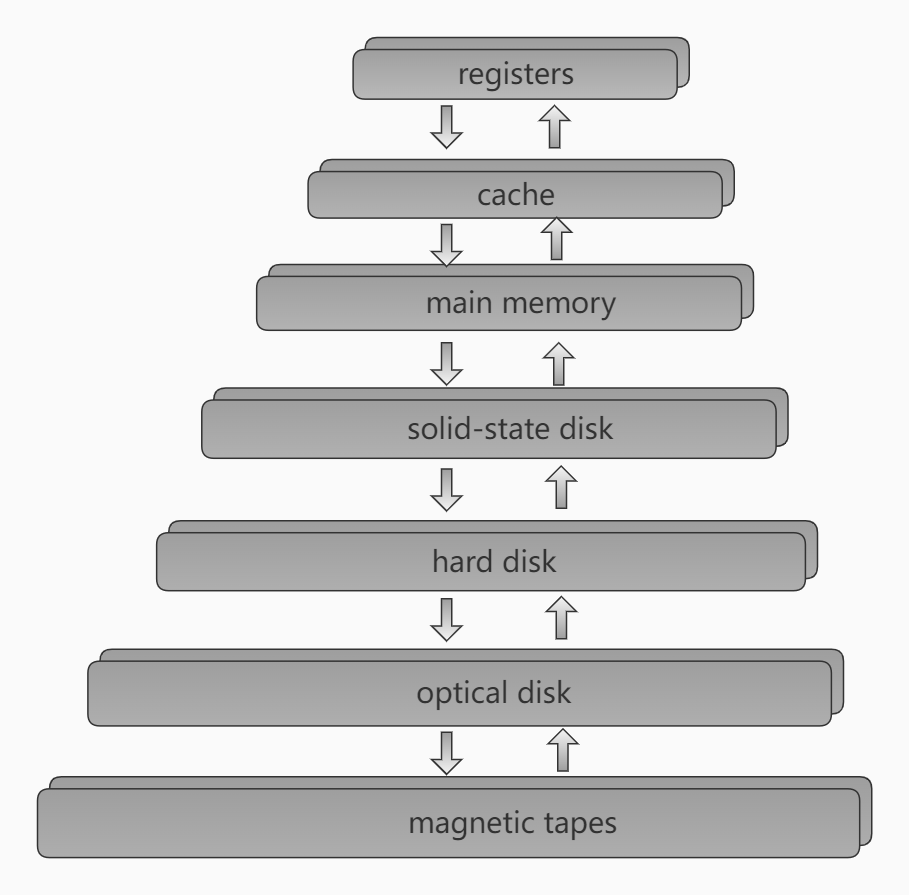
\includegraphics[width=.7\linewidth]{resources/1-18storage_device_hierarchy.jpg} 
\end{figure}
\end{frame}

\begin{frame}{Computer-System Organization}
\framesubtitle{Storage Structure}
\begin{itemize}
\item Main memory --- only large storage media that the CPU can access directly.
\begin{itemize}
\item \alert{Random access}.
\item Typically \alert{volatile}.
\end{itemize}
\item Secondary storage --- extension of main memory that provides large \alert{nonvolatile} storage capacity.
\item Hard disks --- rigid metal or glass platters covered with magnetic recording material.
\begin{itemize}
\item Disk surface is logically divided into tracks, which are subdivided into sectors.
\item The disk controller determines the logical interaction between the device and the computer.
\end{itemize}
\item Solid-state disks --- faster than hard disks, nonvolatile.
\begin{itemize}
\item Various technologies.
\item Becoming more popular.
\end{itemize}
\end{itemize}
\end{frame}

% \begin{frame}{Computer-System Organization}
% \framesubtitle{An Example of I/O Interrupts}
% \begin{figure}
% \begin{minipage}{.32\linewidth}
% 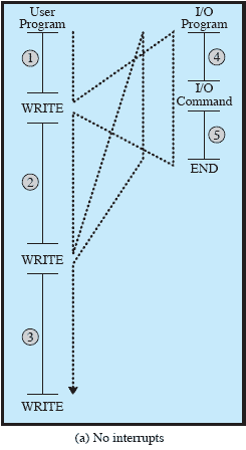
\includegraphics[width=\linewidth]{resources/io_interrupt_a.png} 
% \end{minipage}
% \begin{minipage}{.32\linewidth}
% 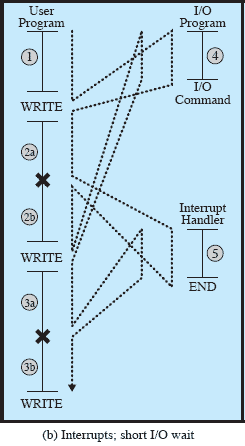
\includegraphics[width=\linewidth]{resources/io_interrupt_b.png} 
% \end{minipage}
% \begin{minipage}{.32\linewidth}
% 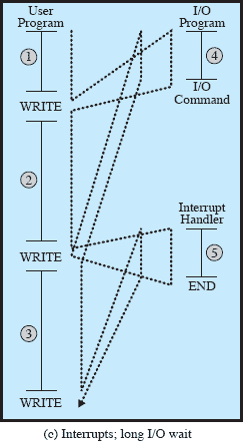
\includegraphics[width=\linewidth]{resources/io_interrupt_c.png} 
% \end{minipage}
% \end{figure}
% \end{frame}

\begin{frame}{Computer-System Organization}
\framesubtitle{I/O Structure --- No Interrupts}
\begin{itemize}
\item After I/O starts, control returns to user program only upon I/O completion
\note[item]{What is control?}
\begin{itemize}
\item Wait instruction idles the CPU.
\item Wait loop (contention for memory access).
\item At most one I/O request is outstanding at a time, no simultaneous I/O processing.
\end{itemize}
\end{itemize}
\end{frame}

\begin{frame}{Computer-System Organization}
\framesubtitle{I/O Structure --- Interrupt Driven}
\begin{itemize}
\item After I/O starts, control returns to user program without waiting for I/O completion
\begin{itemize}
\item \textbf{\alert{System call}} --- request to the OS to allow user to wait for I/O completion.
\item \alert{Device-status table} contains entry for each I/O device indicating its type, address, and state.
\item OS indexes into I/O device table to determine device status and to modify table entry to include interrupt.
\end{itemize}
\item Who returns the control?
\begin{itemize}
\item \alert{Device Driver} for each device controller to manage I/O. Provides uniform interface between controller and kernel.
\end{itemize}
\end{itemize}
\end{frame}

\begin{frame}{Computer-System Organization}
\framesubtitle{I/O Structure --- Direct Memory Access}
\begin{itemize}
\item \textbf{\alert{Direct Memory Access}} Structure
\begin{itemize}
\item Used for high-speed I/O devices able to transmit information at close to memory speeds.
\item Device controller transfers blocks of data from buffer storage directly to main memory without CPU intervention.
\item Only one interrupt is generated per block, rather than the one interrupt per byte.
\end{itemize}
\end{itemize}
\end{frame}

\begin{frame}{Computer-System Organization}
\framesubtitle{How a Modern Computer Works}
\begin{figure}
% TO modify
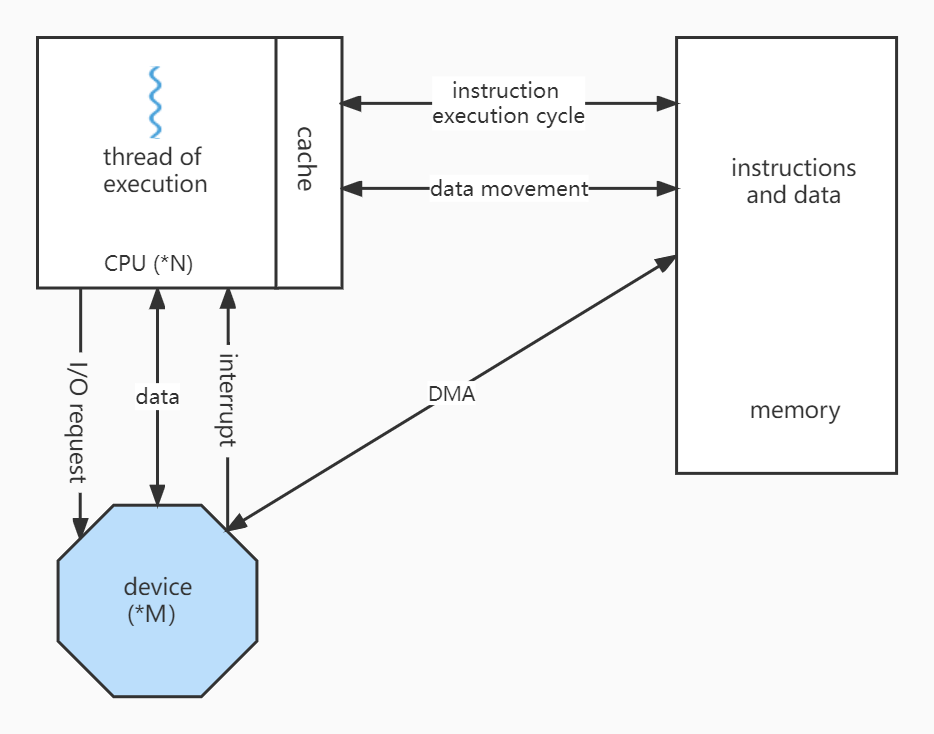
\includegraphics[width=.8\linewidth]{resources/1-23how_a_modern_computer_works.jpg} 
\end{figure}
\end{frame}

\section[3.Architecture]{Computer-System Architecture}
\begin{frame}{Computer-System Architecture}
\begin{itemize}
\item \textcolor{gray}{Most systems use a single general-purpose processor} until 10 years ago.
\begin{itemize}
\item Most systems have special-purpose processors as well.
\end{itemize}
\item \alert{Multiprocessor} systems growing in use and importance.
\begin{itemize}
\item Also known as \alert{parallel systems}, \alert{tightly-coupled systems}.
\item Advantages include:
\begin{enumerate}
\item Increased throughput.
\item Economy of scale.
\item Increased reliability --- graceful degradation or fault tolerance.
\end{enumerate}
\item Two types:
\begin{enumerate}
\item \textbf{\alert{Asymmetric Multiprocessing}} --- each processor is assigned a specific task.
\item \textbf{\alert{Symmetric Multiprocessing}} --- each processor performs all tasks.
\end{enumerate}
\end{itemize}
\end{itemize}
\end{frame}

% \begin{frame}{Computer-System Architecture}
% \framesubtitle{Symmetric Multiprocessing Architecture}
% \begin{figure}
% 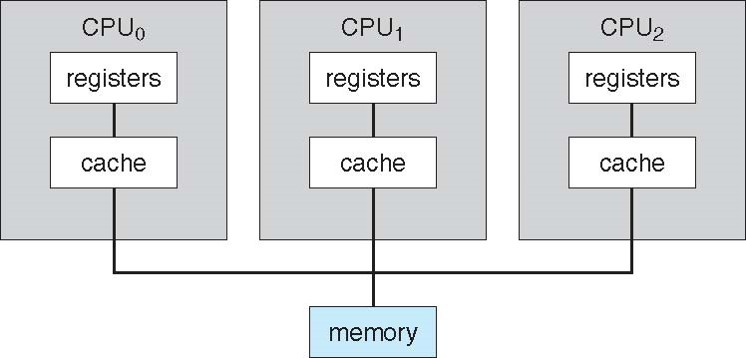
\includegraphics[width=.7\linewidth]{resources/smp_architecture.jpg} 
% \end{figure}
% \end{frame}

\begin{frame}{Computer-System Architecture}
\framesubtitle{A Dual-Core Design}
\begin{itemize}
\item Multi-chip and \alert{multicore}.
\begin{itemize}
\item Why multicore?
\item On-chip communication is faster, uses significantly less power.
\end{itemize}
\item Blade Servers: all in one chassis.
\begin{itemize}
\item Chassis containing multiple separate systems.
\end{itemize}
\end{itemize}
% \begin{figure}
% 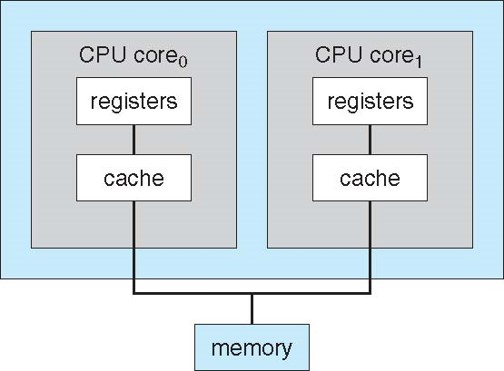
\includegraphics[width=.5\linewidth]{resources/dual_core_design.jpg} 
% \end{figure}
\end{frame}

\begin{frame}{Computer-System Architecture}
\framesubtitle{Clustered Systems}
\begin{itemize}
\item Like multiprocessor systems, but multiple systems working together.
\item \alert{Loosely-coupled systems}.
\begin{itemize}
\item Usually sharing storage via a storage-area network (SAN).
\item Provides a \alert{high-availability} service which survives failures.
\begin{itemize}
\item Asymmetric clustering has one machine in hot-standby mode.
\item Symmetric clustering has multiple nodes running applications, monitoring each other.
\end{itemize}
\item Some clusters are for \alert{high-performance} computing (HPC).
\begin{itemize}
\item Applications must be written to use parallelization.
\end{itemize}
\item Some have distributed lock manager (DLM) to avoid conflicting operations.
\end{itemize}
\end{itemize}
\end{frame}

% \begin{frame}{Computer-System Architecture}
% \framesubtitle{Clustered Systems (contd.)}
% \begin{figure}
% 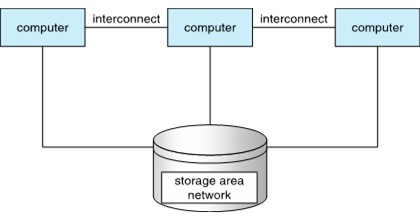
\includegraphics[width=.8\linewidth]{resources/clustered_systems.jpg} 
% \end{figure}
% \end{frame}

\section[4.Structure]{Operating-System Structure}
\begin{frame}{Operating-System Structure}
\framesubtitle{Some History}
\begin{itemize} 
\item No operating system. ($1946\sim 1955$, ENIAC)
\item A typical simple \alert{Batch system} (since 1950s)
\begin{itemize}
\item bring cards to IBM 1401
\item IBM 1401 read cards to tape
\item put tape on IBM 7094 which does computing
\item put tape on IBM 1401 which prints output
\end{itemize}
\end{itemize}
% \begin{figure}
% 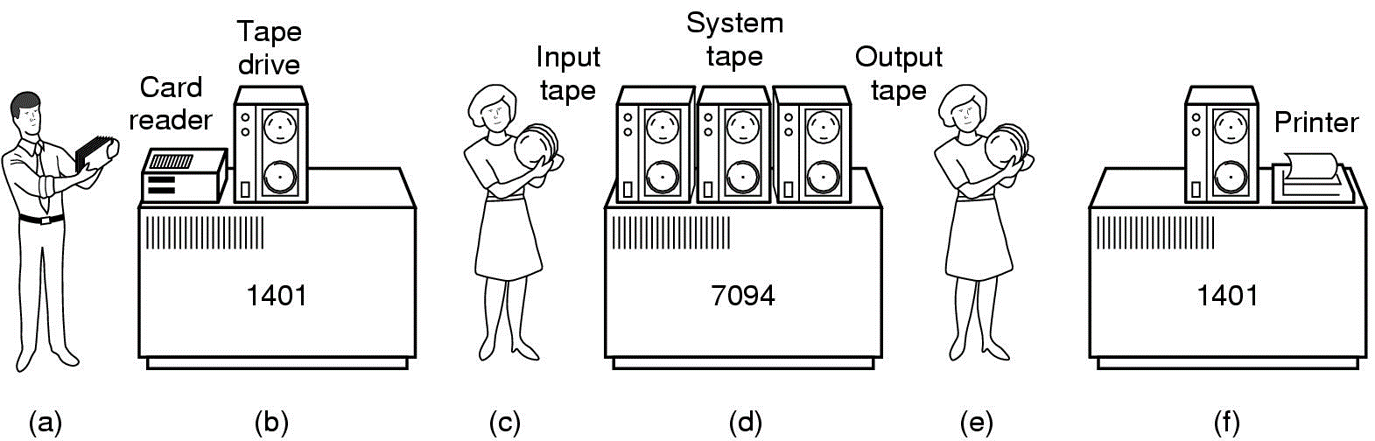
\includegraphics[width=.9\linewidth]{resources/simple_batch_system.png} 
% \end{figure}
\end{frame}

\begin{frame}{Operating-System Structure}
\framesubtitle{Some History (contd.)}
\begin{minipage}{.33\linewidth}
% \begin{figure}
% 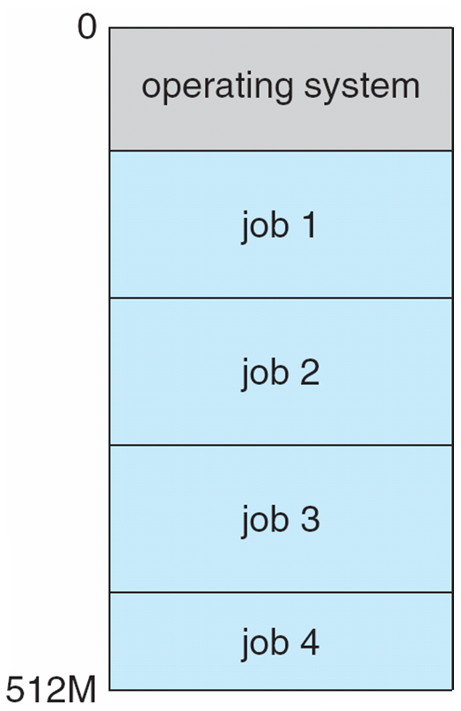
\includegraphics[width=\linewidth]{resources/memory_layout_for_multiprogrammed_system.png} 
% \end{figure}
\begin{table}[]
\centering
\tiny
\begin{tabular}{c|c|l}
\multicolumn{1}{c}{}&\multicolumn{1}{c}{}& \multirow{2}*{$\leftarrow${4GB}}\\
\cline{2-2}
\texttt{0xFFFFFFFF} & \multirow{3}{*}{\textbf{OS}} & \\
& & \\
& & \\
\cline{2-2}
 & & \\
& Job 1 \\
& \\
\cline{2-2}
 & & \\
& Job 2 \\
& \\
\cline{2-2}
 & & \\
& Job 3 \\
& \\
\cline{2-2}
 & & \\
& $\cdots$ \\
\texttt{0x00000000} & & \multirow{2}*{$\leftarrow${0KB}} \\
\cline{2-2}
\end{tabular}
\end{table}
\end{minipage}
\begin{minipage}{.66\linewidth}
\begin{itemize}
\item \textbf{\alert{Multiprogramming}} (Batch system) needed for efficiency. (since 1960s)
\begin{itemize}
\item Single user cannot keep CPU and I/O devices busy at all times.
\item Multiprogramming organizes jobs (code and data) so CPU always has one to execute.
\item A subset of total jobs in system is kept in memory.
\item One job selected and run via \textbf{\alert{job scheduling}} (\textbf{\alert{long term scheduling}}).
\item When it has to wait (for I/O for example), OS switches to another job.
\end{itemize}
\end{itemize}
\end{minipage}
\end{frame}

\begin{frame}{Operating-System Structure}
\framesubtitle{Some History (contd.)}
\begin{itemize}
\item \textbf{\alert{Timesharing}} (multitasking, since 1960s) is logical extension in which CPU switches jobs so frequently that users can interact with each job while it is running, creating \textbf{interactive} computing.
\begin{itemize}
\item \textbf{Response time} should be < 1 second.
\item Each user has at least one program executing in memory --- \textbf{process}.
\item If several jobs ready to run at the same time --- \textbf{\alert{CPU scheduling}} (\textbf{\alert{short term scheduling}}).
\item If processes don't fit in memory, \textbf{swapping} moves them in and out to run.
\item \textbf{Virtual memory} allows execution of processes not completely in memory.
\end{itemize}
\end{itemize}
\end{frame}

\begin{frame}{In Class Exercise}
\framesubtitle{Multiprogramming}
\footnotesize
\begin{itemize}
\item Consider a multiprogramming environment, two programs $A$ and $B$ share the system simultaneously, and run as follows. 
\begin{itemize}
    \item For every 35 min, A runs on CPU for 15 min, then waits for I/O for 20 min.
    \item For every 20 min, B runs on CPU for 10 min, then waits for I/O for 10 min.
\end{itemize}
Suppose $B$ runs first, I/O$_A$ and I/O$_B$ are different devices, and the time of switching between $A$ and $B$ can be ignored. Draw the timeline for these two programs, and calculate CPU utilization within 60 minutes. 
\item What if I/O$_A$ and I/O$_B$ are the same device?
\end{itemize}
% \begin{figure}
% 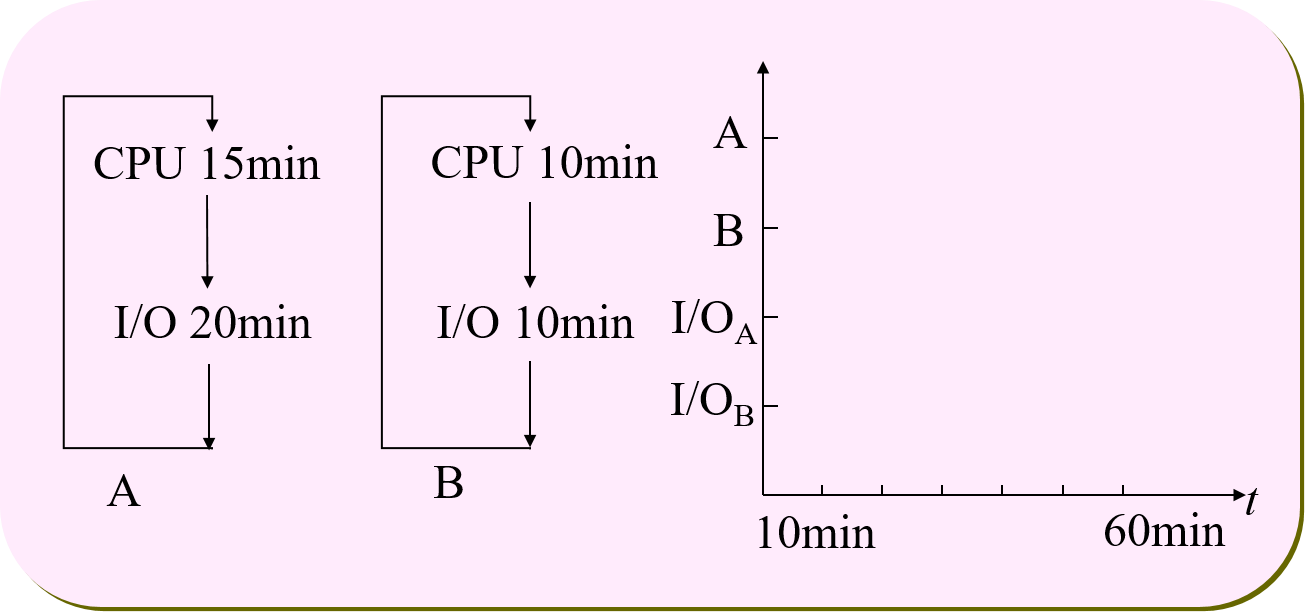
\includegraphics[width=.8\linewidth]{resources/exercise_multiprogramming.png} 
% \end{figure}
\end{frame}

\begin{frame}{In Class Exercise}
\framesubtitle{Key to Multiprogramming}
\footnotesize
Key to Q1: $CPU\ utilization = 50/60 = 83.33\%$\\
v1:
\begin{adjustbox}{scale={.6}}
\begin{ganttchart}[hgrid, vgrid, inline, x unit=3mm, y unit chart=.8cm, y unit title=0.5cm, include title in canvas=false, bar top shift=0, bar height=1, ]{1}{60} 
\ganttgroup{01------05}{01}{05}
\ganttgroup{06------10}{06}{10}
\ganttgroup{11------15}{11}{15}
\ganttgroup{16------20}{16}{20}
\ganttgroup{21------25}{21}{25}
\ganttgroup{26------30}{26}{30}
\ganttgroup{31------35}{31}{35}
\ganttgroup{36------40}{36}{40}
\ganttgroup{41------45}{41}{45}
\ganttgroup{46------50}{46}{50}
\ganttgroup{51------55}{51}{55}
\ganttgroup{56------60}{56}{60}\\
\ganttbar{A}{11}{25}
\ganttbar{A}{56}{60}\\
\ganttbar{B}{1}{10}
\ganttbar{B}{26}{35}
\ganttbar{B}{46}{55}\\
\ganttbar{I/O$_A$}{26}{45}\\
\ganttbar{I/O$_B$}{11}{20}
\ganttbar{I/O$_B$}{36}{45}
\ganttbar{I/O$_B$}{56}{60}
\end{ganttchart}
\end{adjustbox}
v2:
\begin{adjustbox}{scale={.6}}
\begin{ganttchart}[hgrid, vgrid, inline, x unit=3mm, y unit chart=.8cm, y unit title=0.5cm, include title in canvas=false, bar top shift=0, bar height=1, ]{1}{60} 
\ganttgroup{01------05}{01}{05}
\ganttgroup{06------10}{06}{10}
\ganttgroup{11------15}{11}{15}
\ganttgroup{16------20}{16}{20}
\ganttgroup{21------25}{21}{25}
\ganttgroup{26------30}{26}{30}
\ganttgroup{31------35}{31}{35}
\ganttgroup{36------40}{36}{40}
\ganttgroup{41------45}{41}{45}
\ganttgroup{46------50}{46}{50}
\ganttgroup{51------55}{51}{55}
\ganttgroup{56------60}{56}{60}\\
\ganttbar{A}{11}{25}
\ganttbar{A}{46}{60}\\
\ganttbar{B}{1}{10}
\ganttbar{B}{26}{35}\\
\ganttbar{I/O$_A$}{26}{45}\\
\ganttbar{I/O$_B$}{11}{20}
\ganttbar{I/O$_B$}{36}{45}
\end{ganttchart}
\end{adjustbox}
\end{frame}

\begin{frame}{In Class Exercise}
\framesubtitle{Key to Multiprogramming}
\footnotesize
Key to Q2: $CPU\ utilization = 50/60 = 83.33\%$\\
\begin{adjustbox}{scale={.6}}
\begin{ganttchart}[hgrid, vgrid, inline, x unit=3mm, y unit chart=.8cm, y unit title=0.5cm, include title in canvas=false, bar top shift=0, bar height=1, ]{1}{60} 
\ganttgroup{01------05}{01}{05}
\ganttgroup{06------10}{06}{10}
\ganttgroup{11------15}{11}{15}
\ganttgroup{16------20}{16}{20}
\ganttgroup{21------25}{21}{25}
\ganttgroup{26------30}{26}{30}
\ganttgroup{31------35}{31}{35}
\ganttgroup{36------40}{36}{40}
\ganttgroup{41------45}{41}{45}
\ganttgroup{46------50}{46}{50}
\ganttgroup{51------55}{51}{55}
\ganttgroup{56------60}{56}{60}\\
\ganttbar{A}{11}{25}
\ganttbar{A}{46}{60}\\
\ganttbar{B}{1}{10}
\ganttbar{B}{26}{35}\\
\ganttbar{I/O$_A$}{26}{45}
\ganttbar{I/O$_B$}{11}{20}
\ganttbar{I/O$_B$}{46}{55}
\end{ganttchart}
\end{adjustbox}
\end{frame}

\section[5.Operations]{Operating-System Operations}
\begin{frame}{Operating-System Operations}
\framesubtitle{Interrupt Driven (hardware and software)}
\begin{itemize}
\item Hardware interrupt by one of the devices.
\item Software interrupt (\textbf{\alert{exception}} or \textbf{\alert{trap}}):
\begin{itemize}
\item Software error (e.g., division by zero).
\item Request for operating system service.
\item Other process problems include infinite loop, processes modifying each other or the operating system.
\end{itemize}
\end{itemize}
\end{frame}

\begin{frame}{Operating-System Operations}
\framesubtitle{Dual Mode}
\begin{itemize}
\item \textbf{\alert{Dual-mode}} operation allows OS to protect itself and other system components.
\begin{itemize}
\item \textbf{\alert{User mode}} and \textbf{\alert{kernel mode}}.
\item \alert{Mode bit} provided by hardware.
\begin{itemize}
\item Provides ability to distinguish when system is running user code or kernel code.
\item Some instructions designated as \textbf{\alert{privileged}}, only executable in kernel mode.
\item \textbf{\alert{System call}} changes mode to kernel, return from call resets it to user.
\end{itemize}
\end{itemize}
\item Increasingly CPUs support multi-mode operations.
\begin{itemize}
\item i.e., \alert{virtual machine manager} (\alert{VMM}) mode for guest \alert{VMs}.
\end{itemize}
\end{itemize}
\end{frame}

% \begin{frame}{Operating-System Operations}
% \framesubtitle{Dual Mode (contd.)}
% \centering
% Transition from User to Kernel Mode
% \begin{figure}
% 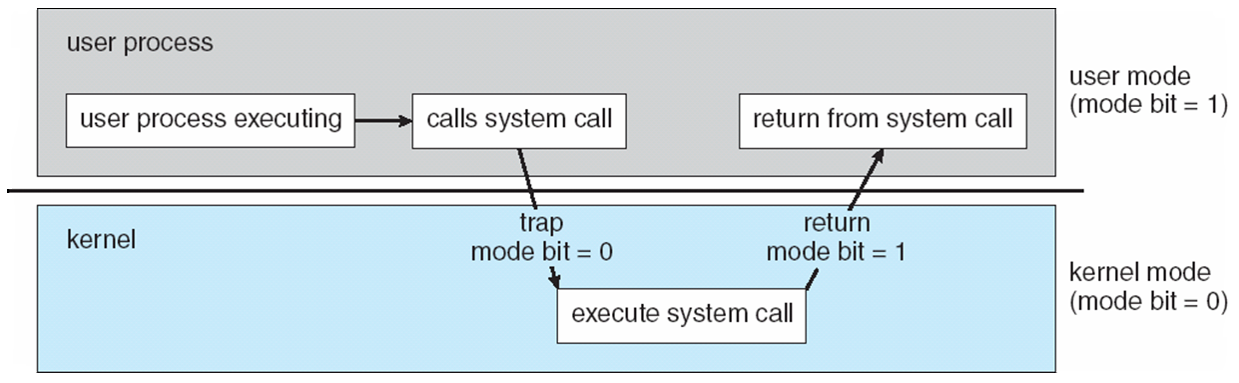
\includegraphics[width=\linewidth]{resources/transition_from_user_to_kernel_mode.png} 
% \end{figure}
% \end{frame}

\begin{frame}{Operating-System Operations}
\framesubtitle{Timer}
\begin{itemize}
\item \textbf{\alert{Timer}} to prevent infinite loop / process hogging resources.
\begin{itemize}
\item Timer is set to interrupt the computer after some time period.
\item Keep a counter that is decremented by the physical clock.
\item Operating system set the counter (privileged instruction).
\item When counter zero generate an interrupt.
\item Set up before scheduling process to regain control or terminate program that exceeds allotted time.
\end{itemize}
\end{itemize}
\end{frame}

\begin{frame}{Operating-System Operations}
\framesubtitle{What Happens When the Computer System is Booting?}
\centering
\scriptsize
\begin{tabular}{l l}
\textbf{OS \MVAt boot}&\textbf{Hardware}\\
\textbf{(kernel mode)}&\\
\hline
initialize trap table&\\
&remember addresses of ...\\
&\quad system call handler\\
&\quad timer handler\\
&\quad illegal instruction handler\\
start interrupt timer&\\
&start timer; interrupt after $X$ ms\\
\end{tabular}
\end{frame}

\begin{frame}{Operating-System Operations}
\framesubtitle{What Happens When the Computer System is Running?}
\centering
\scriptsize
\begin{tabular}{l l l}
\textbf{OS \MVAt run}&\textbf{Hardware}&\textbf{Program}\\
\textbf{(kernel mode)}&&\textbf{(user mode)}\\
\hline
to start process $A$:&&\\
\quad \emph{return-from-trap} (into $A$)&&\\
&move to \emph{user mode}&\\
&&process $A$ runs:\\
&&\quad fetch instruction\\
&&\quad execute instruction\\
&&$\cdots$\\
&timer interrupt&\\
&move to \emph{kernel mode}&\\
&jump to interrupt handler&\\ 
\end{tabular}
\end{frame}

\section[6.Functions]{Operating-System Functions}
\begin{frame}{Operating-System Functions}
\footnotesize
\begin{itemize}
    \item User interface, \textcolor{blue}{in Chapter 2}
    \item CPU management (or \alert{Process management}), \textcolor{blue}{in Chapter 3 $\sim$ 7}
    \begin{itemize}
    \scriptsize
        \item Interrupt handling and management
        \item CPU scheduling
        \item Context switch (save \& restore)
    \end{itemize}
    \item \alert{Memory management}, \textcolor{blue}{in Chapter 8 $\sim$ 9}
    \begin{itemize}
    \scriptsize
        \item Physical memory allocation and deallocation
        \item Address translation (logical $\Leftrightarrow$ physical)
        \item Memory virtualization 
    \end{itemize}
    \item \alert{Storage management}, \textcolor{blue}{in Chapter 10 $\sim$ 12}
    \begin{itemize}
    \scriptsize
        \item Storage space allocation
        \item File \& directory management
    \end{itemize}
    \item Device management, \textcolor{blue}{in Chapter 13}
    \item \textcolor{gray}{Protection and security}, \textcolor{blue}{in Chapter 14 $\sim$ 15}
\end{itemize}
\end{frame}

\begin{frame}{Process/Memory/Storage Management}
\framesubtitle{Too Many Terms?}
\begin{itemize}
\item Just remember three key ideas for now:
\begin{itemize}
\item \textbf{\alert{Virtualization}}: The OS takes a physical resource (such as the processor, or memory, or a disk) and transforms it into a more general, powerful, and easy-to-use virtual form of itself.
\item \textbf{\alert{Concurrency}}: Many problems arise, and must be addressed, when working on many things at once (i.e., concurrently) in the same program.
\item \textbf{\alert{Persistence}}: The OS makes information persist, despite computer crashes, disk failures, or power outages.
\end{itemize}
\end{itemize}
\end{frame}





% \begin{frame}{Process Management}
% \framesubtitle{Processes}
% \begin{itemize}
% \item A process is a program in execution. It is a unit of work within the system. Program is a \alert{passive} entity, process is an \alert{active} entity.
% \item Process needs resources to accomplish its task.
% \begin{itemize}
% \item CPU, memory, I/O, files
% \item Initialization data
% \end{itemize}
% \item Process termination requires reclaim of any reusable resources.
% \item Single-threaded process has one \alert{program counter} specifying location of next instruction to execute.
% \item Multi-threaded process has one program counter per thread.
% \item Typically system has many processes, some user, some operating system running concurrently on one or more CPUs.
% \end{itemize}
% \end{frame}

% \begin{frame}{Process Management}
% \framesubtitle{Process Management Activities}
% \begin{itemize}
% \item The operating system is responsible for the following activities in connection
% with process management:
% \begin{itemize}
% \item Scheduling processes and threads on the CPUs.
% \item Creating and deleting both user and system processes.
% \item Suspending and resuming processes.
% \item Providing mechanisms for process synchronization.
% \item Providing mechanisms for process communication.
% \end{itemize}
% \end{itemize}
% \end{frame}

% \begin{frame}{Memory Management}
% \begin{itemize}
% \item To execute a program, all (or part) of the instructions must be in memory.
% \item All (or part) of the data that is needed by the program must be in memory.
% \item Memory management determines what is in memory and when.
% \begin{itemize}
% \item Optimizing CPU utilization and computer response to users.
% \end{itemize}
% \item Memory management activities:
% \begin{itemize}
% \item Keeping track of which parts of memory are currently being used and by whom.
% \item Deciding which processes (or parts thereof) and data to move into and out of memory.
% \item Allocating and deallocating memory space as needed.
% \end{itemize}
% \end{itemize}
% \end{frame}

% \begin{frame}{Storage Management}
% \begin{itemize}
% \item OS provides a uniform, logical view of information storage.
% \item Abstracts physical properties to logical storage unit --- \textbf{\alert{file}}.
% \item Each medium is controlled by a device (disk drive, tape drive).
% \begin{itemize}
% \item Varying properties include access speed, capacity, data-transfer rate, access method (sequential or random).
% \end{itemize}
% \item File-System management
% \begin{itemize}
% \item Files usually organized into \textbf{\alert{directories}}.
% \item Access control on most systems to determine who can access what.
% \item OS activities include:
% \begin{itemize}
% \item Creating and deleting files and directories.
% \item Primitives to manipulate files and directories.
% \item Mapping files onto secondary storage.
% \item Backup files onto stable (non-volatile) storage media.
% \end{itemize}
% \end{itemize}
% \end{itemize}
% \end{frame}

% \begin{frame}{Storage Management}
% \framesubtitle{Mass-Storage Management}
% \begin{itemize}
% \item Usually disks used to store data that does not fit in main memory or data that must be kept for a ``long'' period of time.
% \item Proper management is of central importance.
% \item Entire speed of computer operation hinges on disk subsystem and its algorithms.
% \item OS activities:
% \begin{itemize}
% \item Free-space management.
% \item Storage allocation.
% \item Disk scheduling.
% \end{itemize}
% \item Some storage need not be fast.
% \begin{itemize}
% \item Tertiary storage includes optical storage, magnetic tape.
% \item Still must be managed --- by OS or applications.
% \item Varies between WORM (write-once, read-many-times) and RW (read-write).
% \end{itemize}
% \end{itemize}
% \end{frame}

% \begin{frame}{Storage Management}
% \framesubtitle{Caching}
% \begin{itemize}
% \item Important principle, performed at many levels in a computer (in hardware, operating system, software).
% \item Information in use copied from slower to faster storage temporarily.
% \item Faster storage (cache) checked first to determine if information is there.
% \begin{itemize}
% \item If it is, information used directly from the cache (fast).
% \item If not, data copied to cache and used there.
% \end{itemize}
% \item Cache smaller than storage being cached.
% \begin{itemize}
% \item Cache management important design problem.
% \item Cache size and replacement policy.
% \end{itemize}
% \end{itemize}
% \end{frame}

% \begin{frame}{Storage Management}
% \framesubtitle{Performance of Various Levels of Storage}
% \begin{figure}
% 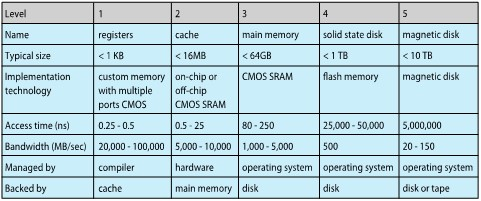
\includegraphics[width=\linewidth]{resources/performance_of_storage.jpg} 
% \end{figure}
% \end{frame}

% \begin{frame}{Storage Management}
% \framesubtitle{Migration of data ``A'' from Disk to Register}
% \begin{itemize}
% \item Multitasking environments must be careful to use most recent value, no matter where it is stored in the storage hierarchy.
% \item Multiprocessor environment must provide \alert{cache coherency} in hardware such that all CPUs have the most recent value in their cache.
% \item Distributed environment situation even more complex.
% \begin{itemize}
% \item Several copies of a datum can exist.
% \end{itemize}
% \end{itemize}
% \begin{figure}
% 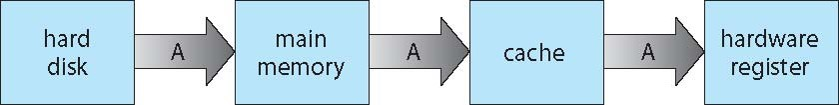
\includegraphics[width=.8\linewidth]{resources/migration_of_data_A.jpg} 
% \end{figure}
% \end{frame}

% \begin{frame}{Storage Management}
% \framesubtitle{I/O Subsystem}
% \begin{itemize}
% \item One purpose of OS is to hide peculiarities of hardware devices from the user.
% \item I/O subsystem consists of:
% \begin{itemize}
% \item Memory management of I/O including \textbf{\alert{buffering}} (storing data temporarily while it is being transferred), \textbf{\alert{caching}} (storing parts of data in faster storage for performance), \textbf{\alert{spooling}} (the overlapping of output of one job with input of other jobs).
% \item General device-driver interface.
% \item Drivers for specific hardware devices.
% \end{itemize}
% \end{itemize}
% \end{frame}

% \begin{frame}{Protection and Security}
% \begin{itemize}
% \item \textbf{\alert{Protection}} --- any mechanism for controlling access of processes or users to resources defined by the OS.
% \item \textbf{\alert{Security}} --- defense of the system against internal and external attacks.
% \begin{itemize}
% \item Huge range, including denial-of-service, worms, viruses, identity theft, theft of service.
% \end{itemize}
% \item Systems generally first distinguish among users, to determine who can do what.
% \begin{itemize}
% \item User identities (\alert{user IDs}, security IDs) include name and associated number, one per user.
% \item User ID then associated with all files, processes of that user to determine access control.
% \item Group identifier (\alert{group ID}) allows set of users to be defined and controls managed, then also associated with each process, file.
% \item \alert{Privilege escalation} allows user to change to effective ID with more rights.
% \end{itemize}
% \end{itemize}
% \end{frame}

\section[7.Misc.]{Other Issues}
\begin{frame}{Kernel Data Structures}
\framesubtitle{You Should Have Known the Concepts of ...}
\begin{itemize}
\item arrays, lists, stacks, and queues,
\item trees,
\item hash functions and maps,
\item bitmaps.
\end{itemize}
\end{frame}

% \section{Computing Environments}
% \begin{frame}{Computing Environments}
% \framesubtitle{Traditional Computing}
% \begin{itemize}
% \item Stand-alone general purpose machines.
% \item But blurred as most systems interconnect with others (i.e., the Internet).
% \item Portals provide web access to internal systems.
% \item Network computers (thin clients) are like Web terminals.
% \item Mobile computers interconnect via wireless networks.
% \item Networking becoming ubiquitous – even home systems use firewalls to protect home computers from Internet attacks.
% \end{itemize}
% \end{frame}

% \begin{frame}{Computing Environments}
% \framesubtitle{Mobile Computing}
% \begin{itemize}
% \item Hand-held smart-phones, tablets, etc.
% \item What is the functional difference between them and a ``traditional'' laptop?
% \item Extra feature --- more OS features (GPS, gyroscope).
% \item Allows new types of apps like augmented reality.
% \item Use IEEE 802.11 wireless, or cellular data networks for connectivity.
% \item Leaders are \alert{Apple iOS} and \alert{Google Android}.
% \end{itemize}
% \end{frame}

% \begin{frame}{Computing Environments}
% \framesubtitle{Distributed Systems}
% \begin{itemize}
% \item Collection of separate, possibly heterogeneous, systems networked together.
% \begin{itemize}
% \item Network is a communications path, TCP/IP most common.
% \begin{itemize}
% \item Local Area Network (LAN)
% \item Wide Area Network (WAN)
% \item Metropolitan Area Network (MAN)
% \item Personal Area Network (PAN)
% \end{itemize}
% \end{itemize}
% \item Network Operating System provides features (such as file sharing) between systems across network.
% \begin{itemize}
% \item Communication scheme allows systems to exchange messages.
% \item Illusion of a single system.
% \end{itemize}
% \end{itemize}
% \end{frame}

% \begin{frame}{Computing Environments}
% \framesubtitle{Client-Server Computing}
% \begin{itemize}
% \item Dumb terminals supplanted by smart PCs.
% \item Many systems now \alert{servers}, responding to requests generated by \alert{clients}.
% \begin{itemize}
% \item Compute-server system provides an interface to client to request services (i.e., database).
% \item File-server system provides interface for clients to store and retrieve files.
% \end{itemize}
% \end{itemize}
% \begin{figure}
% 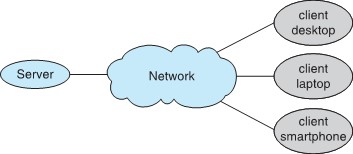
\includegraphics[width=.7\linewidth]{resources/client_server.jpg} 
% \end{figure}
% \end{frame}

% \begin{frame}{Computing Environments}
% \framesubtitle{Peer-to-Peer Computing}
% \begin{minipage}{.39\linewidth}
% \begin{figure}
% 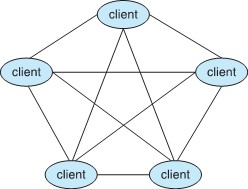
\includegraphics[width=\linewidth]{resources/peer_to_peer.jpg} 
% \end{figure}
% \end{minipage}
% \begin{minipage}{.6\linewidth}
% \begin{itemize}
% \item Does not distinguish clients and servers.
% \begin{itemize}
% \item Instead all nodes are considered peers.
% \item May each act as client, server or both.
% \item Node must join P2P network.
% \begin{itemize}
% \item Registers its service with central lookup service on network, or
% \item Broadcast request for service and respond to requests for service via discovery protocol.
% \end{itemize}
% \item Examples include Napster and Gnutella, Voice over IP (VoIP) such as Skype .
% \end{itemize}
% \end{itemize}
% \end{minipage}
% \end{frame}

% \begin{frame}{Computing Environments}
% \framesubtitle{Virtualization}
% \begin{itemize}
% \item Allows operating systems to run applications within other OSes.
% \begin{itemize}
% \item Vast and growing industry.
% \end{itemize}
% \item \alert{Emulation} used when source CPU type different from target type (i.e. PowerPC to Intel x86).
% \begin{itemize}
% \item Generally slowest method.
% \item When computer language not compiled to native code --- \alert{Interpretation}.
% \end{itemize}
% \item \alert{Virtualization} --- OS natively compiled for CPU, running guest OSes also natively compiled.
% \begin{itemize}
% \item Consider VMware running WinXP guests, each running applications, all on native WinXP host OS.
% \item \alert{Virtual machine manager} (\alert{VMM}) provides virtualization services.
% \end{itemize}
% \end{itemize}
% \end{frame}

% \begin{frame}{Computing Environments}
% \framesubtitle{Virtualization (contd.)}
% \begin{figure}
% 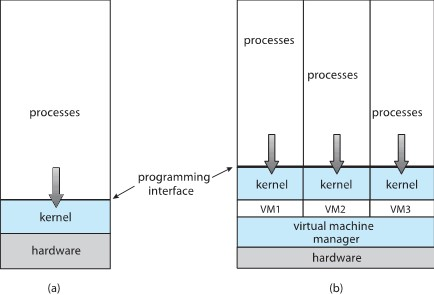
\includegraphics[width=.8\linewidth]{resources/virtualization.jpg} 
% \end{figure}
% \end{frame}

% \begin{frame}{Computing Environments}
% \framesubtitle{Cloud Computing}
% \begin{itemize}
% \footnotesize
% \item Delivers computing, storage, apps as a service across a network.
% \item Logical extension of virtualization because it uses virtualization as the base for its functionality.
% \item Many types:
% \begin{itemize}
% \footnotesize
% \item \alert{Public cloud} --- available via Internet to anyone willing to pay.
% \item \alert{Private cloud} --- run by a company for the company's own use.
% \item \alert{Hybrid cloud} --- includes both public and private cloud components.
% \item Software as a Service (\alert{SaaS}) --- one or more applications available via the Internet (i.e., word processor).
% \item Platform as a Service (\alert{PaaS}) --- software stack ready for application use via the Internet (i.e., a database server).
% \item Infrastructure as a Service (\alert{IaaS}) --- servers or storage available over Internet (i.e., storage available for backup use).
% \end{itemize}
% \end{itemize}
% \end{frame}

% \begin{frame}{Computing Environments}
% \framesubtitle{Real-Time Embedded Systems}
% \begin{itemize}
% \item Real-time embedded systems most prevalent form of computers.
% \begin{itemize}
% \item Vary considerable, special purpose, limited purpose OS, \alert{real-time OS}.
% \item Use expanding.
% \end{itemize}
% \item Many other special computing environments as well.
% \begin{itemize}
% \item Some have OSes, some perform tasks without an OS.
% \end{itemize}
% \item Real-time OS has well-defined fixed time constraints.
% \begin{itemize}
% \item Processing must be done within constraint.
% \item Correct operation only if constraints met.
% \end{itemize}
% \end{itemize}
% \end{frame}

%\section{Open-Source Operating Systems}
\begin{frame}{Open-Source Operating Systems}
\begin{itemize}
\item Operating systems made available in source-code format rather than just binary closed-source.
\item Counter to the copy protection and Digital Rights Management (DRM) movement.
\item Started by Free Software Foundation (FSF), which has ``copyleft'' GNU Public License (GPL).
\item Examples include GNU/Linux and BSD UNIX (including core of Mac OS X), and many more.
\item Can use VMM like VMware Player (Free on Windows), Virtualbox (open source and free on many platforms - available @ \url{http://www.virtualbox.com}) .
\begin{itemize}
\item Use to run guest operating systems for exploration.
\end{itemize}
\end{itemize}
\end{frame}

\begin{frame}{openEuler Operating System}
\begin{itemize}
    \item Xv6
    \begin{itemize}
        \item Xv6 documentation (PDF):     \href{https://seunic-my.sharepoint.cn/:b:/g/personal/101011912_seu_edu_cn/EYdcF-SBSqNOlamCf9zcEbUBweJItRDGhnVuyC4JkNWSbw?e=iPfoTS}{\texttt{link}}
        \item Xv6 codes (PDF):     \href{https://seunic-my.sharepoint.cn/:b:/g/personal/101011912_seu_edu_cn/ESodUyrBhS5GmDMV6cCE4ZYBzddjcv8Dn9LgDdSJ1TILFA?e=EGIP6r}{\texttt{link}}
    \item Xv6 structure (mind): \href{https://docs.qq.com/mind/DR1FTZXpzamFYRnhx}{\texttt{link}}
    \end{itemize}
    \item EulerOS 
    \begin{itemize}
        \item A commercial Linux distribution developed by Huawei based on CentOS source code for enterprise applications.
        \item Available @ \url{https://openeuler.org/en/}
    \end{itemize} 
\end{itemize}
    
\end{frame}


\begin{frame}{After Class Exercise}
\begin{itemize}
    \item Exercise 1.19, p51.
    \begin{itemize}
        \item What is the purpose of interrupts? How does an interrupt differ from a trap? Can traps be generated intentionally by a user program? If so, for what purpose?
    \end{itemize}
\end{itemize}
\end{frame}

\end{document}
